\documentclass{article}

%
% 引入模板的style文件
%
\usepackage{homework}

\setCJKmainfont{SimSun}[AutoFakeBold] %宋体加粗
\setCJKsansfont{SimHei}[AutoFakeBold] %黑体加粗


\usepackage{minted} %配合minted宏包进行好看的高亮
\usepackage{currfile} %配合minted宏包进行好看的高亮
\usepackage{caption} %配合minted宏包进行好看的高亮
\usepackage{tcolorbox} %配合minted宏包进行好看的高亮
\usepackage{xcolor} %配合minted宏包进行好看的高亮
\tcbuselibrary{skins} %配合minted宏包进行好看的高亮
\tcbuselibrary{minted} %配合minted宏包进行好看的高亮
\usemintedstyle{paraiso-dark} %配合minted宏包进行好看的高亮
\usepackage{framed} 


%
% 封面
%


\title{
	
\includegraphics[width=0.6\textwidth]{images/title/ucas_logo 1.pdf}\\
    \vspace{1in}
    \textmd{\textbf{\hmwkClass}}\\
	\textmd{\Large{\textbf{\hmwkClassID}}}\\
    \textmd{\textbf{\hmwkTitle}}\\
    \normalsize\vspace{0.1in}\large{\hmwkCompleteTime }\\
    \vspace{0.1in}\large{\textit{\hmwkClassInstructor\ }}\\
    \vspace{1in}
	
\includegraphics[width=0.25\textwidth]{images/title/Cyber.jpg}\\
	\vspace{1in}
}

\author{
	\hmwkAuthorName \\ 
	\hmwkAuthorStuID \\
	\hmwkAuthorInst \\
	\hmwkAuthorzhuanye \\
	\hmwkAuthorfangxiang
	}
\date{}

\renewcommand{\part}[1]{\textbf{\large Part \Alph{partCounter}}\stepcounter{partCounter}\\}


%
% 正文部分
%
\begin{document}


\maketitle


%\include{chapters/ch01}
%\include{chapters/ch02}
%\include{chapters/ch03}
%\include{chapters/ch04}
%\include{chapters/ch05}


\pagebreak

\begin{homeworkProblem}
	设有$n$个顾客同时等待一项服务. 顾客$i$需要的服务时间为$t_i, 1 \leq i\leq n$. 应该如何安排$n$个顾客的服务次序才能使总的等待时间达到最小? 总的等待时间是各顾客等待服务的时间的总和. 试给出你的做法的理由(证明).
	\\

	\solution 我们使用贪心算法求解该问题, 具体的\textbf{贪心策略}为: \textbf{服务时间较短的优先安排}. 假设调度$f$的顺序为$i_1,i_2,\cdots, i_n$, 那么$i_k$的等待时间为$\displaystyle \sum_{j=1}^{k-1}{t_{i_j}}$, 总的等待时间为$\displaystyle T\left( f \right) =\sum_{i=1}^n{\left( n-i \right) t_{i_j}}$. 根据贪心策略, 需要先排序使得$t_1\leq t_2 \leq \cdots \leq t_n$, 按照$1,2,\cdots,n$的顺序安排服务. 则调度$f^{\ast}$的总等待时间为$\displaystyle T\left( f^{\ast} \right) =\sum_{i=1}^n{\left( n-i \right) t_i}$.
	于是我们可以给出对应的算法伪码:
	\begin{algorithm}[H]
		\begin{algorithmic}[1]
		\Require{服务时间的数组$T[1,\cdots,n]=[t_1,t_2,\cdots,t_n]$}
		\Ensure{调度$f$, $f(i)$为第$i$个顾客的开始服务时刻, $1\leq i\leq n$}
		\State \textbf{sort}($T.\text{begin}()$, $T.\text{end}()$); \Comment{按照服务时间从小到大的顺序排列}
		\State $f(1):=0$;
		\For{$i:=2$ to $n$}
			\State $f(i):=f(i-1)+t_{i-1}$;
		\EndFor
		\State \Return $f$;
		\State \textbf{end \{Service\}}
		\end{algorithmic}
		\caption{\textbf{Service}算法}
		\label{alg:Service}
	\end{algorithm}
	由于\textbf{算法主要在于排序}, 故其最坏情况下的时间复杂度为$O(n\log n)$. 
	
	下面证明: \textbf{对任何输入, 对服务时间短的顾客优先安排将得到最优解.}
	\begin{proof}
		\textbf{交换论证:} 不妨设$t_1\leq t_2\leq \cdots t_n$, 算法的调度$f$结果为$1,2,\cdots,n$. 如果它不是最优的, 则存在最优调度$f^*$, 设其最早第$k$项作业$i_k$与$f$不同, 即$f^*:1,2,\cdots,k-1,i_k,i_{k+1},\cdots,i_n$. 则必有$t_{i_{k}}\geq t_k$. 现将$f^*$中的作业$k$与作业$i_k$置换, 得到调度$f^{**}:1,2,\cdots,k,i_{k+1},\cdots,i_k,\cdots,i_n$. 其中$i_k$位置为$j$, 则$j>k,t_{i_{k}}\geq t_k$. 则有$$T\left( f^* \right) -T\left( f^{**} \right) =\left( j-k \right) \left( t_{i_k}-t_k \right) \ge 0
		$$
		说明$f^{**}$也是最优调度, 且它与$f$不同的次序项后移了一位. 重复最多$n$步, 则可得$f$最优.
	\end{proof}
\end{homeworkProblem}

\pagebreak

\begin{homeworkProblem}
	字符$a\sim h$出现的频率分布恰好是前8个Fibonacci数, 它们的Huffman编码是什么? 将结果推广到$n$个字符的频率分布恰好是前$n$个Fibonacci数的情形. Fibonacci数的定义为: $F_0=1,F_1=1,F_n=F_{n-2}+F_{n-1}(n\geq 1)$.
	\\
	
	\solution 对应的Huffman树如下图\ref{fig:Huffman树}所示. 故可知Huffman编码为
	\begin{align}
		h:0,\,g:10,\,f:110,\,e:1110,\,d:11110,\,c:111110,\,b:1111110,\,a:1111111
	\end{align}
	\begin{figure}[H]  % 这里记得用[H]
		\centering
		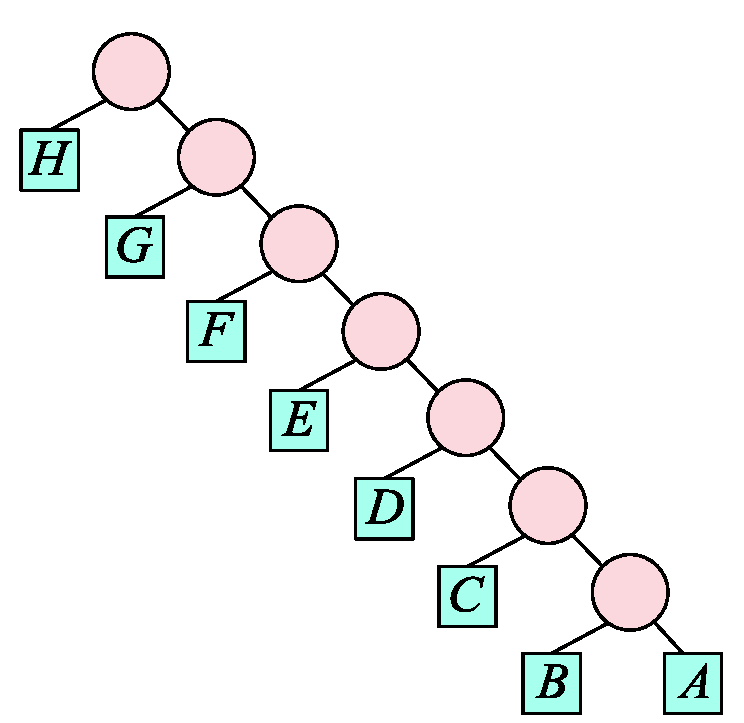
\includegraphics[width=0.35\textwidth]{images/title/Huffman树.pdf}
		\caption{Huffman树}
		\label{fig:Huffman树}
	\end{figure}
	为了推广, 需要先证明一个结论: 设$f_i(i\geq 1)$为Fibonacci数列, 则
	\begin{align}
		\sum_{i=1}^k{f_i}\le f_{k+2} \label{inequ1}
	\end{align}
	\begin{proof}
		采用数学归纳法: 当$k=1$时, 命题显然成立; 假设$k=n$时命题成立, 则$k=n+1$时, 则有
		\begin{align}
			\sum_{i=1}^{n+1}{f_i}=\sum_{i=1}^n{f_i}+f_{n+1}\le f_{n+2}+f_{n+1}=f_{n+3}
		\end{align}
		于是$\forall k\in \mathbb{N}^{\ast}$, 不等式(\ref{inequ1})都成立.
	\end{proof}
	因此根据上述结论, 前$k$个字符合并后子树的根权值小于等于第$k+2$个Fibonacci数. 根据Huffman算法, 他将继续参加与第$k+1$个字符的合并. 因此$n$个字符的Huffman编码按照频数从小到大依次为
	\begin{align}
		\underset{n-1\text{个}1}{\underbrace{11\cdots 1}},\, \underset{n-2\text{个}1}{\underbrace{11\cdots 10}}, \, \underset{n-3\text{个}1}{\underbrace{11\cdots 0}}, \, \cdots , \, 10,\, 0
	\end{align}
	即第$i(i>1)$个字母的编码为$\underset{n-i\text{个}1}{\underbrace{11\cdots 10}}$.
\end{homeworkProblem}

\pagebreak

\begin{homeworkProblem}
	设$p_1,p_2,\cdots,p_n$是准备存放到长为$L$的磁带上的$n$个程序, 程序$p_i$需要的带长为$a_i$. 设$\displaystyle \sum_{i=1}^n{a_i}>L$, 要求选取一个能放在带上的程序的最大子集合(即其中含有最多个数的
	程序)$Q$. 构造$Q$的一种贪心策略是按$a_i$的非降次序将程序计入集合.

	(1). 证明这一策略总能找到最大子集$Q$, 使得$\displaystyle \sum_{p_i\in Q}{a_i}\le L$;

	(2). 设$Q$是使用上述贪心算法得到的子集合, 磁带的利用率可以小到何种程度?

	(3). 试说明(1)中提到的设计策略不一定能得到使$\displaystyle \sum_{p_i\in Q}{a_i}/L$(即磁带的利用率)取最大值的子集合.
	\\

	\solution 
	
	(1).
	\begin{proof}
		还是采用\textbf{交换论证}: 易知只要存放程序名称相同(不管次序)的任何方法都是同样的解. 不妨设最优解为$\text{OPT}=\left\{ i_1,i_2,\cdots ,i_j \right\} ,i_1<i_2<\cdots <i_j,j < n	$. 如果
		\begin{align}
			\left\{ i_1,i_2,\cdots ,i_j \right\} =\left\{ 1,2,\cdots ,j \right\}
		\end{align}
		那么算法的解就是最优解. 假设$\left\{ i_1,i_2,\cdots ,i_j \right\} \ne \left\{ 1,2,\cdots ,j \right\}$, 设$i_1=1,i_2=2,\cdots, i_{t-1}=t-1,i_t>t$. 用$t$替换$i_t$, 那么得到的解$I^{\ast}$占用的存储空间与解OPT占用空间的差值为
		\begin{align}
			S\left( I^{\ast} \right) -S\left( \text{OPT} \right) =a_t-a_{i_t}\le 0
		\end{align}
		因此$I^{\ast}$也是最优解, 但是它比解OPT减少了一个标号不相等的程序. 对于解OPT, 从第一个标号不等的程序开始, 至多经过$j$次替换, 就得到最优解$\left\{ 1,2,\cdots ,j \right\}$. 显然算法的时间复杂度为
		\begin{align}
			T\left( n \right) =O\left( n\log n \right) +O\left( n \right) =O\left( n\log n \right) 
		\end{align}
	\end{proof}
	
	(2). 磁带的利用率最小可以小到0, 比如$\forall 1\leq i\leq n,a_i>L$.

	(3). 按照题中的贪心策略虽然能够保障所装的程序最多, 但对应的空间利用率不一定最大. 具体例子为: 设$\left\{ a_1,a_2,\cdots a_s \right\} $为$Q$的最大子集, 可能会有: 用$a_{s+1}$替换$a_s$, 子集合变为$\left\{ a_1,a_2,\cdots a_{s-1},a_{s+1} \right\} $并且满足$\displaystyle \sum_{k=1}^{s-1}{a_k}+a_{s+1}<L$. 虽然程序个数仍为$s$个, 但利用率却增加了. 因此上述贪心策略并不一定能求得使利用率最大化的最优解.

	(4). 如果要求磁带利用率最大, 这个问题的本质上是0-1背包问题, 每个程序相当于物品, 其重量和价值就是所需要的存储带长, 背包的重量限制等于磁带容量$L$. 可以使用动态规划(DP)算法来解决: 设$F_k\left( y \right) $表示考虑前$k$个程序, 磁带空间为$y$时的最大存储量. 递推方程为
	\begin{align}
		F_k\left( y \right) =\begin{cases}
			\max \left\{ F_{k-1}\left( y \right) ,F_{k-1}\left( y-a_k \right) +a_k \right\} , a_k\le y\le L\\
			F_{k-1}\left( y \right) , a_k>y\\
		\end{cases}
	\end{align}
	其中$k>0$且$F_0\left( y \right) =0 \left( 0\le y\le L \right) , F_k\left( 0 \right) =0, F_k\left( y \right) =-\infty \left( y<0 \right)$. 可以设定如下标记函数$i_k(y)$用于追踪解:
	\begin{align}
		i_k\left( y \right) =\begin{cases}
			k, \text{若}F_{k-1}\left( y \right) \le F_{k-1}\left( y-a_k \right) +a_k,a_k\le y\le L\left( k>1 \right)\\
			i_{k-1}\left( y \right) , \text{否则}\\
		\end{cases},\,\, i_1\left( y \right) =\begin{cases}
			1, \text{若}y\ge a_1\\
			0, \text{否则}\\
		\end{cases}
	\end{align}
	该DP算法在最坏情形下的时间复杂度为$T(n)=O(nL)$.
\end{homeworkProblem}



\pagebreak

\begin{homeworkProblem}
	写出Huffman编码的伪代码, 并编程实现. 
	\\

	\solution 伪代码见如下算法\ref{alg:HuffmanCode}:
	\begin{algorithm}[H]
		\begin{algorithmic}[1]
		\Require{待编码的数组$A[1,\cdots,n]$}
		\Ensure{数组$A$的Huffman编码}
		\State \textbf{local} $h$; \Comment{最小化堆, 内含元素为结点类型, 堆初始为空}
		\State \textbf{int} $i$;
		\State \textbf{Node} $p,q,r$; \Comment{结点数据结构, 内含数值以及分别指向左、右儿子的两个指针}
		\For{$i=1$; $i<=n$; $i$++} \Comment{将数组$A$中的所有元素插入堆}
			\State $\textbf{Insert}(h,A[i])$;
		\EndFor
		\While{$|h|>1$} \Comment{$h$元素个数大于1}
			\State $p=\textbf{DeleteMin}(h)$; $q=\textbf{DeleteMin}(h)$; \Comment{移除最小的两个结点}
			\State $r=p+q$; $r
			.\text{left} = \text{min}(p, q)$; $r.\text{right} = \text{max}(p, q)$; \Comment{构造新的结点$r$, 其值为 $p,q$值之和}
			\State $\textbf{Insert}(h,r)$; \Comment{将$r$插入堆$h$中}
		\EndWhile
		\State $p=\textbf{DeleteMin}(h)$; \Comment{取出最后一个结点, 此节点即为Huffman树的根节点}
		\State \textbf{end \{HuffmanCode\}}
		\end{algorithmic}
		\caption{\textbf{HuffmanCode}算法}
		\label{alg:HuffmanCode}
	\end{algorithm}
\end{homeworkProblem}



\begin{homeworkProblem}
	举出反例证明: 本章开始例1贪心规则找零钱算法(目标: 零币数量最少;规则: 尽量先找币值大的), 在零钱种类不合适时, 贪心算法结果不正确.
	\\

	\solution 比如, 如果提供找零的面值是11,5,1, 找零15.
	使用贪心算法找零方式为11+1+1+1+1, 需要五枚硬币. 而最优解为5+5+5, 只需要3枚硬币.
\end{homeworkProblem}


\pagebreak

\begin{homeworkProblem}
	设有一条边远山区的道路$AB$, 沿着道路$AB$分布着$n$所房子. 这些房子到$A$的距离分别是$d_1,d_2,\cdots,$
	$d_n(d_1<d_2<\cdots<d_n)$. 为了给所有房子的用户提供移动电话服务, 需要在这条道路上设置一些基站. 为了保证通讯质量, 每所房子应该位于距离某个基站的4km范围内. 设计一个算法找基站的位置, 并且使得基站的总数最少, 并证明算法的正确性.
	\\

	\solution 使用贪心法, 令$a_1,a_2,\cdots$表示基站的位置. 贪心策略为: 首先令$a_1=d_1+4$. 对$d_2,d_3,\cdots,d_n$依次检查, 找到下一个不能被该基站覆盖的房子. 如果$d_k\leq a_1+4$但$d_{k+1}>a_1+4$, 那么第$k+1$个房子不能被基站覆盖, 于是取$a_2=d_{k+1}+4$作为下一个基站的位置. 照此下去, 直到检查完$d_n$为止. 伪代码见如下算法\ref{alg:Location}:
	\begin{algorithm}[H]
		\begin{algorithmic}[1]
		\Require{距离数组$d[1,\cdots,n]=[d_1,d_2,\cdots,d_n]$, 满足$d[1]<d[2]<\cdots<d[n]$}
		\Ensure{基站位置的数组$a$}
		\State $a[1]:=d[1]+4$; $k:=1$;
		\For{$j=2$; $j<=n$; $j$++}
			\If{$d[j]>a[k]+4$}
				\State $a[\text{++}k]:=d[j]+4$;
			\EndIf
		\EndFor
		\State \Return $a$;
		\State \textbf{end \{Location\}}
		\end{algorithmic}
		\caption{\textbf{Location}算法}
		\label{alg:Location}
	\end{algorithm}
	\textbf{结论: 对任何正整数$k$, 存在最优解包含算法前$k$步选的的基站位置.}
	\begin{proof}
		$k=1$, 存在最优解包含$a[1]$. 如若不然, 有最优解OPT, 其第一个位置是$b[1]$且$b[1]\neq a[1]$, 那么$d_1-4\leq b[1] <d_1+4=a[1]$. $b[1]$覆盖的是距离在$[d_1,b[1]+4]$之间的房子. $a[1]$覆盖的是距离在$[d_1,a[1]+4]$的房子. 因为$b[1]<a[1]$, 且$b[1]$覆盖的房子都在$a[1]$覆盖的区域内, 故用$a[1]$替换$b[1]$得到的仍是最优解;

		假设对于$k$, 存在最优解$A$包含算法前$k$步选择的基站位置, 即
		\begin{align}
			A=\left\{ a\left[ 1 \right] ,a\left[ 2 \right] ,\cdots ,a\left[ k \right] \right\} \cup B
		\end{align}
		其中$a[1],a[2],\cdots,a[k]$覆盖了距离为$d_1,d_2,\cdots,d_j$的房子. 那么$B$是关于$L=\left\{ d_{j+1},d_{j+2},\cdots ,d_n \right\} $的最优解. 否则, 存在关于$L$的更优解$B^{\ast}$, 那么用$B^{\ast}$替换$B$就会得到$A^{\ast}$且$\left| A^{\ast} \right|<\left| A \right|$, 这与$A$是最优解相矛盾. 根据归纳假设可得知$L$有一个最优解$B'=\left\{ a\left[ k+1 \right] ,\cdots \right\} ,\left| B' \right|=\left| B \right|$. 于是
		\begin{align}
			A'=\left\{ a\left[ 1 \right] ,a\left[ 2 \right] ,\cdots ,a\left[ k \right] \right\} \cup B'=\left\{ a\left[ 1 \right] ,a\left[ 2 \right] ,\cdots ,a\left[ k \right] ,a\left[ k+1 \right] ,\cdots \right\} 
		\end{align}
		且$\left| A' \right|=\left| A \right|$, 故$A'$也是最优解, 从而命题对于$k+1$也成立. 故根据数学归纳法可知, 对任何正整数$k$命题都成立.
	\end{proof}
	算法的关键操作是for循环, 而循环体內部的操作都是常数时间, 因此算法在最坏情况下的时间复杂度为$O(n)$.
\end{homeworkProblem}

\pagebreak

\begin{homeworkProblem}
	有$n$个进程$p_1,p_2,..,p_n$, 进程$p_i$的开始时间为$s[i]$, 截止时间为$d[i]$. 可以通过检测程序Test来测试正在运行的进程, Test每次测试时间很短, 可以忽略不计, 即如果Test在时刻$t$测试, 那么它将对满足$s[i]\leq t \leq d[i]$的所有进程同时取得测试数据. 问: 如何安排测试时刻, 使得对每个进程至少测试一次, Test测试的次数达到最少? 设计算法并证明正确性, 分析算法复杂度.
	\\

	\solution \textbf{贪心策略}: 将进程按照ddl进行排序. 取第1个进程的ddl作为第一个测试点, 然后顺序检查后续能够被这个测试点检测的进程 (这些进程的开始时间$\leq$测试点), 直到找到下一个不能被测试到的进程为止. 伪码见如下算法\ref{alg:Test}:
	\begin{algorithm}[H]
		\begin{algorithmic}[1]
		\Require{开始时间的数组$s[1,\cdots,n]$, 截止时间的数组$d[1,\cdots,n]$}
		\Ensure{数组$t$: 顺序选定的测试点构成的数组}
		\State 将进程按照$d[i]$递增的顺序进行排序(使得$d[1]\leq d[2]\leq \cdots \leq d[n]$);
		\State $i:=1$; $t[i]:=d[1]$; $j:=2$ \Comment{第一个测试点是最早结束进程的ddl}
		\While{$j\leq n$ $\&\&$ $s[j]\leq t[i]$} \Comment{检查进程$j$是否可以在时刻$t[i]$被测试}
			\State $j$++;
		\EndWhile
		\If{$j>n$}
			\State \Return $t$;
		\Else
			\State $t[\text{++}i]:=d[j\text{++}]$, \textbf{goto} 3; \Comment{找到待测进程中结束时间最早的进程$j$}
		\EndIf
		\State \textbf{end \{Test\}}
		\end{algorithmic}
		\caption{\textbf{Test}算法}
		\label{alg:Test}
	\end{algorithm}
	\textbf{结论: 对于任意正整数$k$, 存在最优解包含算法前$k$步选择的测试点.}
	\begin{proof}
		$k=1$时, 设$S=\left\{ t\left[ i_1 \right] ,t\left[ i_2 \right] ,\cdots \right\} $是最优解, 不妨设$t\left[ i_1 \right] <t\left[ 1 \right]$. 设$p_u$是在时刻$t[i_1]$被测到的任意进程, 那么$s(u)\leq t[i_1] \leq d[u]$, 从而有
		\begin{align}
			s\left[ u \right] \le t\left[ i_1 \right] <t\left[ 1 \right] =d\left[ 1 \right] \le d\left[ u \right] 
		\end{align}
		因此$p_u$也可以在$t[1]$时刻被测试. 于是在$S$中用$t[1]$替换掉$t[i_1]$后也可得到一个最优解.

		假设对于任意$k$, 算法在前$k$步选择了$k$个测试点$t[1],t[i_2],\cdots,t[i_k]$且存在最优解
		\begin{align}
			T=\left\{ t\left[ 1 \right] ,t\left[ i_2 \right] ,\cdots ,t\left[ i_k \right] \right\} \cup T'
		\end{align}
		设算法前$k$步选择的测试点不能测到的进程构成集合$Q\subseteq P$, 其中$P$为全体进程集合. 不难证明$T'$是子问题$Q$的最优解\footnote{反证法: 假设$T'$不是子问题$Q$的最优解, 则会推出$T$不是最优解, 显然矛盾.}. 根据归纳假设可得知, $\exists Q$的最优解$T^{\ast}$包含测试点$t[i_{k+1}]$, 即
		\begin{align}
			T^{\ast}=\left\{ t\left[ i_{k+1} \right] \right\} \cup T''
		\end{align}
		因此有
		\begin{align}
			\left\{ t\left[ 1 \right] ,t\left[ i_2 \right] ,\cdots ,t\left[ i_k \right] \right\} \cup T^{\ast}=\left\{ t\left[ 1 \right] ,t\left[ i_2 \right] ,\cdots ,t\left[ i_{k+1} \right] \right\} \cup T''
		\end{align}
		也是原问题的最优解, 根据归纳法可知命题成立.
	\end{proof}
	算法的时间复杂度为$T\left( n \right) =O\left( n\log n \right) +O\left( n \right) =O\left( n\log n \right)$.
	\newpage
\end{homeworkProblem}

\pagebreak

\begin{homeworkProblem}
	设有作业集合$J=\{1,2,\cdots,n\}$, 每项作业的加工时间都是1, 所有作业的截止时间是$D$. 若作业$i$在$D$之后完成, 则称为被延误的作业, 需赔偿罚款$m(i)(i=1,2,\cdots,n)$, 这里$D$和$m(i)$都是正整数, 且$n$项$m(i)$彼此不等. 设计一个算法求出使总罚款最小的作业调度算法, 证明算法的正确性并分析时间复杂度.
	\\

	\solution \textbf{贪心策略:} 优先安排前$D$个罚款最多的作业. 正确性证明需要利用交换论证的方法, 先给出以下结论:

	\textbf{结论:} 设作业调度$f$的安排次序是$\left< i_1,i_2,\cdots ,i_n \right> $, 那么罚款为
	\begin{align}
		F\left( f \right) =\sum_{k=D+1}^n{m\left( i_k \right)}
	\end{align}
	\begin{proof}
		显然最优调度没有空闲时间, 不妨假设作业是连续安排的. 因为每项作业的加工时间都是1, 再截止时间D之前可以完成$D$项作业. 只有在$D$之后安排的$n-D$项作业(即$i_{D+1},i_{D+2},\cdots,i_{n}$都是被罚款的作业).
	\end{proof}
	根据上述结论可以推出: 令$S$是$n-D$项罚款最少的作业构成的集合.

	(1). 对于$S$(或$J\backslash S$)中的作业$i$和$j$, 交换$i,j$的加工顺序不影响总罚款;

	(2). 对于作业$i$和$j$, $m(i)<m(j)$, 调度$f$将$i$安排在$D$之前, $j$安排在$D$之后, 那么交换作业$i$和$j$得到的调度$g$, 则$g$的罚款会减少, 这是因为
	\begin{align}
		F(g) - F(f) = m(i) - m(j) < 0
	\end{align}
	根据上述分析可以看出, 把罚款最小的$n-D$项作业安排在最后会使得总罚款金额达到最小.

	于是可以设计出以下算法\ref{alg:Work}
	\begin{algorithm}[H]
		\begin{algorithmic}[1]
		\Require{罚款数组$m[1,\cdots,n]$, 作业集合$J$}
		\Ensure{作业调度$f$}
		\State $m^*:=\textbf{Partselect}(m[\quad],n-D)$;
		\State \textbf{Partition}($m[\quad],A,B,m^*$);
		\State $\left\{ i_1,i_2,\cdots ,i_D \right\} :=B$;
		\State $\left\{ i_{D+1},i_{D+2},\cdots ,i_n \right\} :=A+\left\{ m^* \right\}$;
		\State \textbf{end \{Work\}}
		\end{algorithmic}
		\caption{\textbf{Work}算法}
		\label{alg:Work}
	\end{algorithm}
	现在来分析一下这个算法的时间复杂度: 第1行调用了\textbf{PartSelect}算法, 最坏需要$O(n)$的时间; 第2步调用的\textbf{Partition}算法也需要$O(n)$的时间, 故总的时间复杂度为$T(n)=O(n)+O(n)=O(n)$.
\end{homeworkProblem}



% 引用文献
\bibliographystyle{unsrt}  % unsrt:根据引用顺序编号
\bibliography{refs}


\end{document}
